\section{Etherless}
	\subsection{Architecture} % Descrizione dell'architettura utilizzata tra i tre moduli cli, smart e server
	This section describes the overall architecture of \textit{Etherless}. \\
	\textit{Etherless} was developed as a layered architecture consisting of three layers, which are also its main components:
	\begin{itemize}
		\item \textbf{Etherless-cli};
		\item \textbf{Etherless-smart};
		\item \textbf{Etherless-server}.
	\end{itemize}
	Each one of these layers has a specific role and responsibility in managing users' requests, and only interacts with the layer directly below it.
	\begin{figure} [h!]
		\centering
		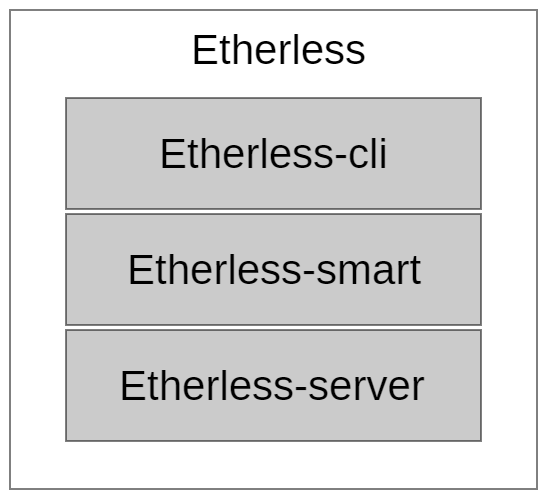
\includegraphics[width=0.7\linewidth]{diagrammi/generali/LayeredArchitecture}
		\caption{Etherless layered architecture}
	\end{figure}
	\pagebreak
	\paragraph{} The product's modules, each one representing a layer, also have a one-way dependency towards the next module.
	\begin{figure} [h!]
		\centering
		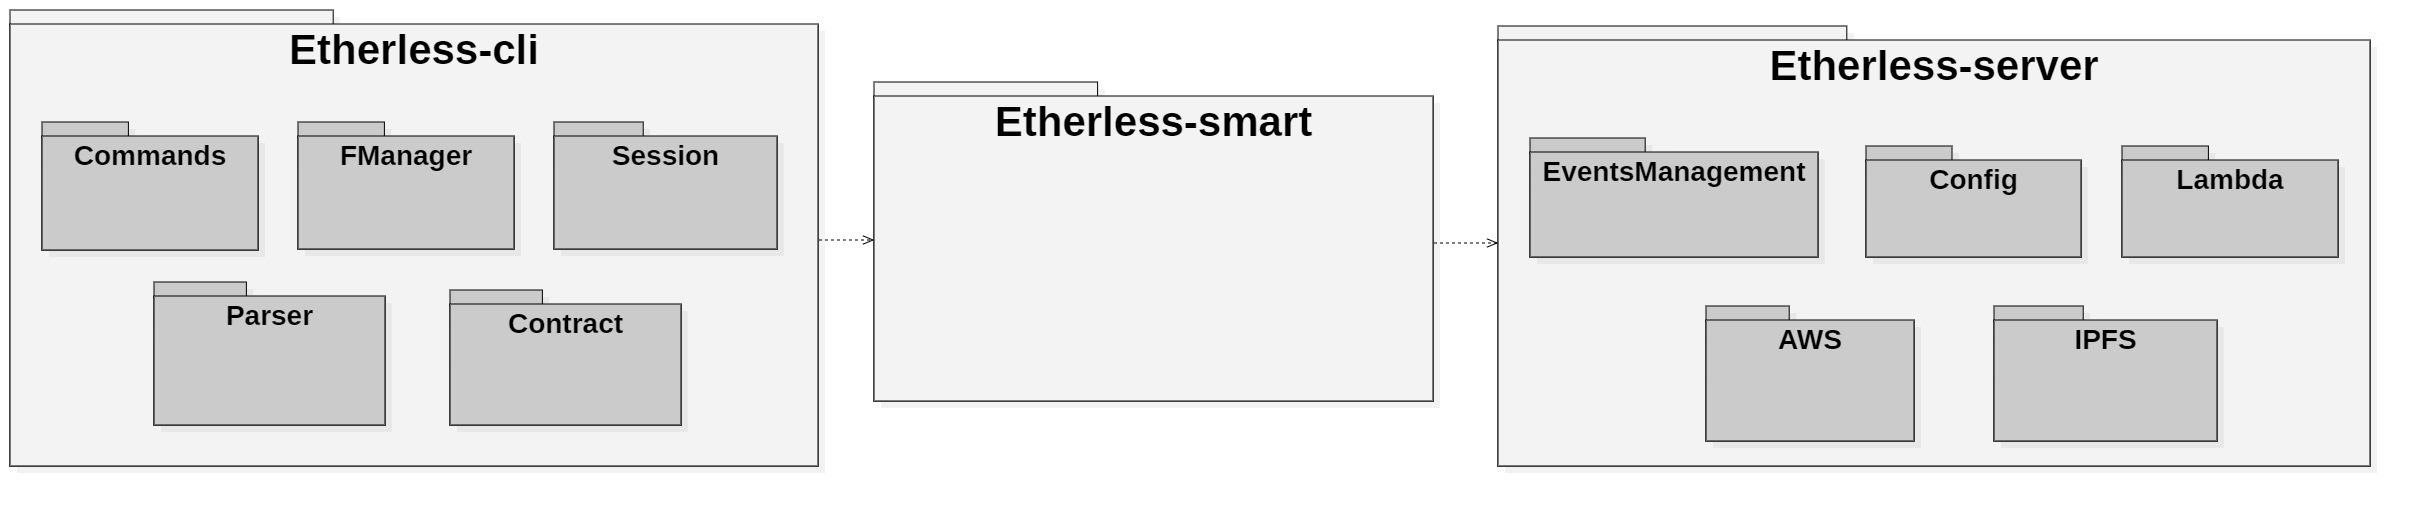
\includegraphics[width=15cm, height=3.5cm]{diagrammi/generali/Etherless_package}
		\caption{Package diagram of the Etherless architecture}
	\end{figure}
	\subsection{Communication} % Descrizione della comunicazione dei tre moduli, per le diverse funzionalità
	Following the layered architecture pattern, the users' requests received by Etherless-cli move from one layer to the layer right below it. Which means that every module has a specific role in the communication:
	\begin{itemize}
		\item \textbf{Etherless-cli}: accepts users' requests, routes them to Etherless-smart and displays information to the user;
		\item \textbf{Etherless-smart}: processes the received requests and forwards them to Etherless-server if needed. Also returns the requests results to Etherless-cli, once they have been completed;
		\item \textbf{Etherless-server}: interacts with AWS Lambda$_{G}$ and other services in order to satisfy the received requests.
	\end{itemize}
	\begin{figure}
		\centering
		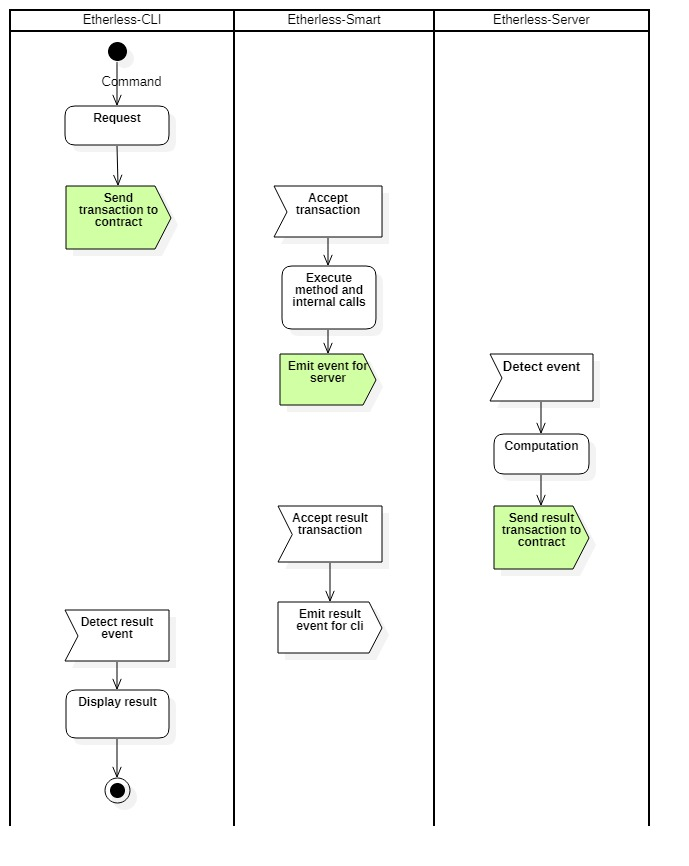
\includegraphics[width=0.9\linewidth]{diagrammi/generali/activity_diag_pattern2}
		\caption{Activity diagram of a request interacting with AWS Lambda$_{G}$.}
	\end{figure}
	Not all types of requests trigger the communication between all three modules. Some types of requests that do not need an interaction with AWS Lambda$_{G}$ itself will be single-handedly completed by Etherless-smart.
	\begin{figure} [h!]
		\centering
		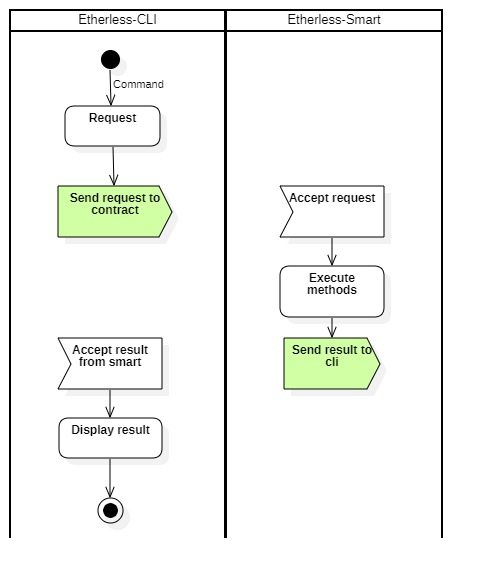
\includegraphics[width=0.8\linewidth]{diagrammi/generali/activity_diag_pattern1}
		\caption{Activity diagram of a request that doesn't interact with AWS Lambda$_{G}$.}
	\end{figure}
	\pagebreak
	\\
